%
% Categorifying the zx-calculus
% Open graphs over Szx
% arXiv v2
%

\documentclass[./1--Catfying_zxCalc--Master.tex]{subfiles} % ./mainfilename.tex
%\input{Catfying_zxCalc--Preamble.tex}

%%%%%%%%%%%%%%%%%%
%%%%%%%%%%%%%%%%%%
% 
\begin{document}
%
%%%%%%%%%%%%%%%%%%
%%%%%%%%%%%%%%%%%%

%%%%%%%%%%%%%%%%%%%%%%
%%%%%%%%%%%%%%%%%%%%%%
% OPEN STRUCTURED GRAPHS
\section{Open graphs over $S_{\text{zx}}$}
\label{sec:OpenGraphsOverSzx}
%%%%%%%%%%%%%%%%%%%%%%
%%%%%%%%%%%%%%%%%%%%%%

Last section, 
we began the process of
modeling the zx-calculus with 
graphs by introducing 
open graphs and fitting them 
into a bicategory $\mathbf{Rewrite}$.  
This overcame the issue of 
graphs lacking inputs and outputs.  
In this section, we  
face a different issue.  
Unlike open graphs,
 $\mathbf{zx}$-morphisms 
have multi-sorted nodes.
In this section, we
equip open graphs with
multi-sorted nodes by
working with a 
slice category of 
$\cat{Graph}$. 
Kissinger used a similar
method to give graphs
multi-sorted nodes in 
his thesis
	\cite{Kissinger_Pictures}.

\begin{defn}
	\label{def:graph over Szx}
	Let $S$ be a graph.  
	By a \emph{graph over $S$}, 
	we mean a graph morphism $G \to S$. 
	A morphism between graphs over $S$ 
	is a graph morphism $G \to G'$ 
	such that the following
	diagram commutes
	\[
	\begin{tikzpicture}
	\node (1) at (-0.5,1) {$G$};
	\node (2) at (0.5,1) {$G'$};
	\node (3) at (0,0) {$S$};
	%
	\path[->,font=\scriptsize,>=angle 90]
	(1) edge (2)
	(1) edge (3)
	(2) edge (3);
	\end{tikzpicture}
	\]
\end{defn} 

Every graph morphism $G \to G'$ contains 
a map between corresponding nodes sets.
The fibre of this map
colors the $G$-nodes 
with the $G'$-nodes.
We illustrate this with the following example.

\begin{ex}
	\label{ex:basic graph over Szx}
	%
	Let $S_{\text{zx}}$ be the graph
	%
	\begin{equation}
	\label{diag:zx struture graph}
	\raisebox{-0.75\height}{
		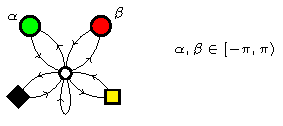
\includegraphics{InclGrphx--slice--graph_S_zx}
	}
	\end{equation}
	%
	We have not drawn 
	the entirety of $S_{\text{zx}}$. 
	The green and red nodes actually
	run through $[-\pi,\pi)$ and 
	all of them have 
	a single arrow to and from node 
	$
	\begin{tikzpicture}
		\node [zxopen] at (0,0) {};
	\end{tikzpicture}
	$. 
	
	Most of the structure of the 
	basic $\mathbf{zx}$-morphisms 
	is captured by graphs over $S_{\text{zx}}$.
	Consider the following graphs over $S_{\text{zx}}$
	\[
	\label{fig:ZX 1cells generators}
		\begin{minipage}{0.33\textwidth}
			\centering
			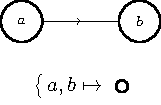
\includegraphics{InclGrphx--slice--wire_over_Szx}
		\end{minipage}
%
		\begin{minipage}{0.34\textwidth}
			\centering
			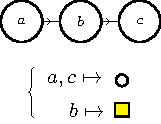
\includegraphics{InclGrphx--slice--Hadamard_over_Szx}
		\end{minipage}
%	
		\begin{minipage}{0.33\textwidth}
			\centering
			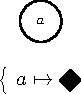
\includegraphics{InclGrphx--slice--diamond_over_Szx}
		\end{minipage}
	\]
	\[
	\begin{minipage}{0.5\textwidth}
		\centering
		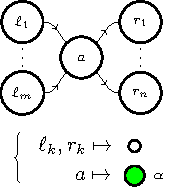
\includegraphics{InclGrphx--slice--green_spider_over_Szx}
	\end{minipage}
	%			\quad \quad \quad \quad
	\begin{minipage}{0.5\textwidth}
		\centering
		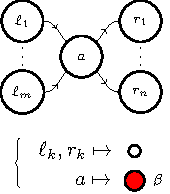
\includegraphics{InclGrphx--slice--red_spider_over_Szx}
	\end{minipage}
	\]
	where the diagrams give the 
	domain of each graph over $S_{\text{zx}}$
	and the map is described directly
	underneath each diagram.
	The behavior of each map
	is determined by the image
	of the nodes
	because there is at most 
	one arrow between any 
	two nodes in $S_{\text{zx}}$.  
	The role played by each node 
	of $S_{\text{zx}}$ in 
	providing our desired structure 
	is evident except, perhaps, 
	for the node
	$
	\begin{tikzpicture}
		\node [zxopen] at (0,0) {};
	\end{tikzpicture}
	$.   
	Observe that four of the 
	basic $\mathbf{zx}$-morphisms 
	have dangling wires on either end.  
	Because edges of directed graphs 
	must be attached to 
	a pair of nodes, 
	we use this node
	to anchor the dangling edges.
\end{ex}

\begin{ex}
	\label{ex:graph over Szx}
	At this point, 
	we can interpret
	the basic zx-diagrams as 
	graphs over $S_{\text{zx}}$. 
	This extends nicely to 
	a translation of any
	$\mathbf{zx}$-morphism, 
	such as
	\[
	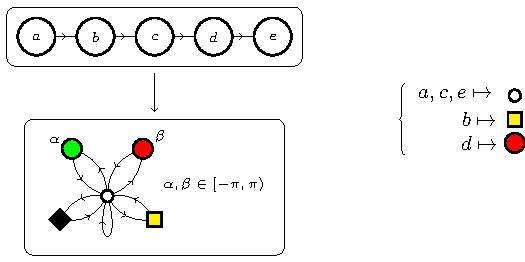
\includegraphics{InclGrphx--example--graph_over_Szx}
	\]
	which corresponds to the $\mathbf{zx}$-morphism 
	\[
	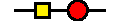
\includegraphics{InclGrphx--example--zx_morphism_as_graph_over_Szx}
	\]
\end{ex}

The graphs over $S_{\text{zx}}$ 
in Examples 
\ref{ex:basic graph over Szx} and
\ref{ex:graph over Szx}
capture most of the structure 
of the basic $\mathbf{zx}$-morphisms.  
The ability to compose is still missing.
Composition becomes possible
with \emph{open graphs over $S_{\text{zx}}$}.
Again, we use cospans 
to make this precise, 
though combining these two structure 
introduces new considerations. 

Start with the slice category 
$\mathbf{Graph} \downarrow S_{\text{zx}}$ 
of graphs over $S_{\text{zx}}$. 
By Theorem 
	\ref{thm:SpCspC is SMCC bicategory}, 
this gives us an SMCC bicategory 
$\mathbf{Sp} ( \mathbf{Csp} 
	( \mathbf{Graph} \downarrow S_{\text{zx}} ) ) $  
within which we want to 
construct a sub-bicategory 
analogous to $\mathbf{Rewrite}$.  
However, there is a problem. 
Recall that the objects of $\mathbf{Rewrite}$ 
have form $N(X)$ where 
	$N \colon \mathbf{Set}_0 \to \mathbf{Graph}$ 
is the functor sending a set 
to the edgeless graph on that set.  
In $\mathbf{Graph}$, 
there is a unique, 
up to isomorphism,
way to be an edgeless graph.
But in $\mathbf{Graph} \downarrow S_{\text{zx}}$, 
there may be many ways
to be edgeless.
This depends on the number of
graph morphisms to $S_{\text{zx}}$. 
For instance, a graph with 
$n$ nodes and no edges 
can be a graph over $S_{\text{zx}}$ 
in $5^n$ ways. 
We rectify this issue by functorially
turning a set into an edgeless graph. 
Recall that $\mathbf{FinSet}_0$ is a
skeleton of $\mathbf{FinSet}$.

\begin{defn}
	\label{def:Nzx functor}
	Define a functor 
		$N_{\text{zx}} \colon \mathbf{FinSet}_0 
			\to 
			\mathbf{Graph} \downarrow S_{\text{zx}}$ 
	by 
		\[
			X \mapsto (N_{\text{zx}}(X) \to S_{\text{zx}})
		\]
	where $N_{\text{zx}}(X)$ is 
	the edgeless graph with 
	nodes $X$ that are 
	constant over 
	$\begin{tikzpicture} 
		\node [zxopen] at (0,0) {}; 
	\end{tikzpicture}$. 
	An \emph{open graph over $S_{\text{zx}}$} 
	is a cospan in 
	$\mathbf{Graph} \downarrow S_{\text{zx}}$ 
	of the form
	\[
		N_{\text{zx}}(X) \to G \gets N_{\text{zx}} (Y).
	\]
\end{defn}

With this definition of
open graphs over $S_{\text{zx}}$, 
we propose the analogue 
to $\mathbf{Rewrite}$. 

\begin{defn}
	Define $\mathbf{zxRewrite}$ 
	to be the symmetric monoidal and 
	compact closed sub-bicategory of 
	$\mathbf{Sp} ( \mathbf{Csp} 
	( \mathbf{Graph} \downarrow S_{\text{zx}} ) ) $  
	that is 1-full and 2-full 
	on objects of the form 
	$N_{\text{zx}} (X)$ for finite sets $X$.  
\end{defn}

Unpacking this definition, 
the 0-cells of $\mathbf{zxRewrite}$ 
are those edgeless graphs over $S_{\text{zx}}$ 
in the image of $N_{\text{zx}}$.  
The 1-cells are exactly 
the open graphs over $S_{\text{zx}}$. 
The 2-cells are the rewritings of
one open graph over $S_{\text{zx}}$ 
into that preserve the inputs and outputs.  
To better understand this bicategory, 
we give an example of 
an open graph over $S_{\text{zx}}$. 
Along with this example, 
we present a new notation 
that allow us to draw the
remaining diagrams 
more compactly.

\begin{ex}
	\label{ex:open graph over Szx}
	Consider the graph over $S_{\text{zx}}$ 
	in Example \ref{ex:graph over Szx}.  
	Make this an open graph as follows:
	\[
		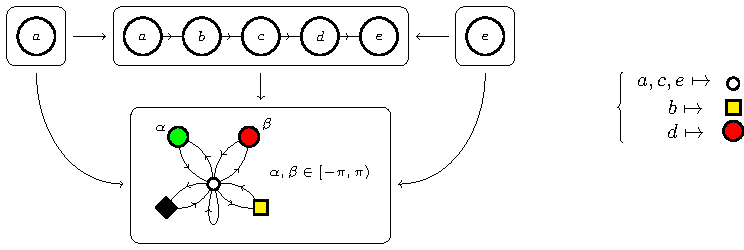
\includegraphics[scale=0.9]{InclGrphx--example--open_graph_over_Szx}
	\]
	There is a single input, 
	node $a$, and 
	a single output, node $e$. 
	Denote this by
	\[
		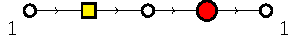
\includegraphics{InclGrphx--example--zx_morphism_as_open_graph_over_Szx}
	\]
	The input nodes are 
	aligned on the far left and 
	the output nodes on the far right.  
	The $1$'s in the corners 
	refer to the cardinality of 
	the input and output node sets.  
	This may seem unnecessary 
	or redundant, 
	but it will clarify 
	several situations arising later on. 
	Thus, we side with consistency 
	and always write the cardinalities.
	Of course, this notation 
	strips a fair amount information 
	regarding the graph morphisms 
	involved in the cospan. 
	However, any missing information 
	should be evident in context.
\end{ex}

Recall that
our interest in 
$\mathbf{Rewrite}$ 
is as an ambient space
in which to generate 
syntactical bicategories 
for graphical languages.
The same is true of
our new bicategory $\mathbf{zxRewrite}$.  
Presently, we are interested in 
1-cells corresponding to 
the basic $\mathbf{zx}$-morphisms 
and 2-cells to the basic relations 
depicted in Figure \ref{fig:ZX equations}.  
We claim that the
bicategory generated by 
these 1-cells and 2-cells 
categorifies $\mathbf{zx}$.
 
%%%%%%%%%%%%%%%%%%
%%%%%%%%%%%%%%%%%%
% 
\end{document}
%
%%%%%%%%%%%%%%%%%%
%%%%%%%%%%%%%%%%%%
